\documentclass{beamer}


\usepackage{graphicx}
\usepackage{amsmath}
\usepackage{amssymb}
\usepackage{algpseudocode}


\title{Reinforcement Learning: Chapter 7 - n-step Bootstrapping}
\subtitle{Based on Sutton and Barto's Book}
\author{Flávio Codeço Coelho}
\date{\today}


\begin{document}


    \frame{\titlepage}


    \begin{frame}
        \frametitle{Outline}
        \tableofcontents
    \end{frame}


    \section{Introduction}
    \begin{frame}
        \frametitle{Introduction}
        \begin{itemize}
            \item Overview of n-step Bootstrapping
            \item Importance in the context of Reinforcement Learning
            \item Main objectives and learning outcomes
        \end{itemize}
    \end{frame}

    \begin{frame}{n-step Bootstrapping}
        \begin{itemize}
            \item Balances between sampling and bootstrapping
            \item Extends one-step TD prediction to use multiple steps
            \item n-step return balances immediate reward and future value
            \item Evaluates the policy over multiple steps
        \end{itemize}
    \end{frame}


    \section{n-step TD prediction}
    \begin{frame}
        \frametitle{n-step TD Prediction}
        \begin{itemize}
            \item Extends one-step TD prediction to use multiple steps
            \item Balance between bootstrapping and sampling
            \item Mathematical formulation:
            $$
            V(s) \leftarrow V(s) + \alpha [G_t^{(n)} - V(s)]
            $$
            \item ($G_t^{(n)}$): n-step return
        \end{itemize}
    \end{frame}

    \begin{frame}
        \frametitle{n-step Return}
        \begin{columns}
            \column{0.5\textwidth}
            \begin{itemize}
                \item Definition of n-step return:
                \begin{multline*}
                    G_{t:t+n} = R_{t+1} + \gamma R_{t+2} + \ldots \\
                    + \gamma^{n-1} R_{t+n} + \gamma^n V_{t+n-1}(S_{t+n})
                \end{multline*}
                \item Balances immediate reward and future value
            \end{itemize}
            \column{0.5\textwidth}
            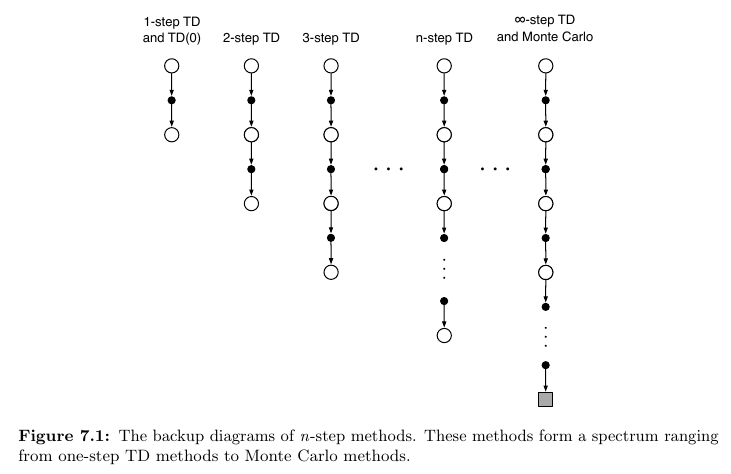
\includegraphics[width=\textwidth]{n-step-return.png}
        \end{columns}
\vspace{20pt}
        Full return, truncated after n steps and then corrected for the
remaining missing terms by $V_{t+n-1}(S_{t+n})$
    \end{frame}

    \begin{frame}{n-step TD Prediction Algorithm}
        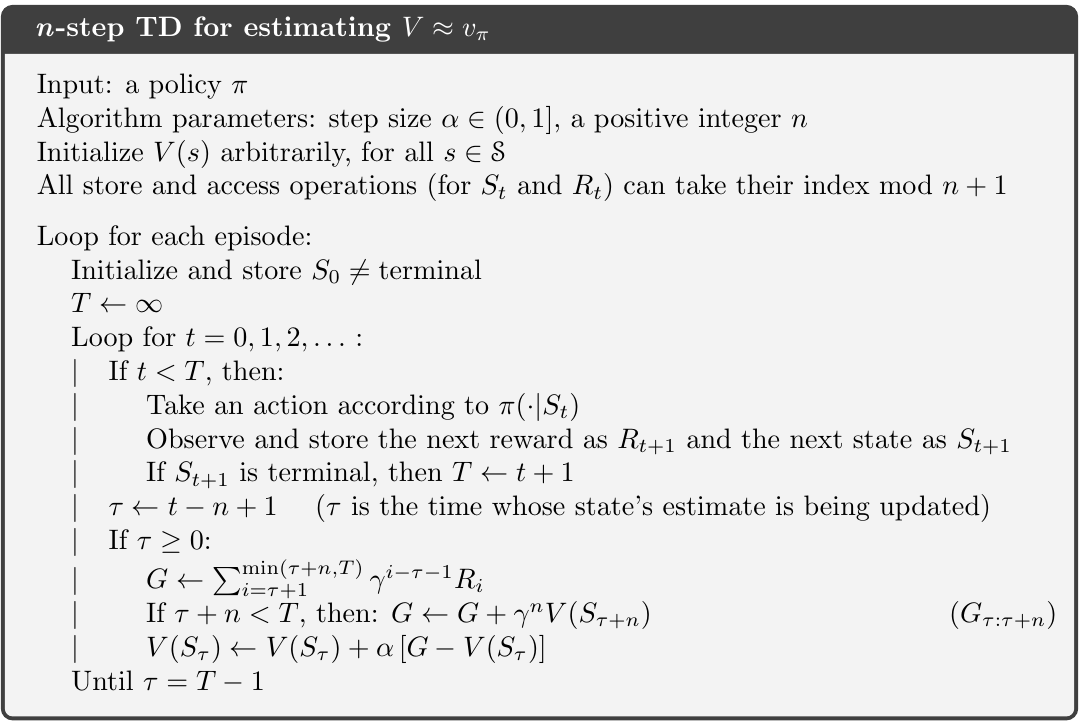
\includegraphics[width=\textwidth]{n-step-td-prediction-alg.png}
     \end{frame}


    \section{n-step SARSA}
    \begin{frame}
        \frametitle{n-step SARSA}
        \begin{itemize}
            \item Extends TD prediction to control using an on-policy method
            \item SARSA: State-Action-Reward-State-Action
            \item Update rule:
            $$
            Q_{t+n}(s,a) = Q_{t+n-1}(s,a) + \alpha \left[G_{t:t+n} - Q_{t+n-1}(s,a)\right]
            $$
        \end{itemize}
    \end{frame}


    \begin{frame}
        \frametitle{n-step Return for SARSA}
        \begin{itemize}
            \item Definition of n-step return for SARSA:
            \begin{multline*}
                G_{t:t+n} = R_{t+1} + \gamma R_{t+2} + \ldots \\
                + \gamma^{n-1} R_{t+n} + \gamma^n Q_{t+n-1}(S_{t+n}, A_{t+n})
            \end{multline*}
        \end{itemize}
    \end{frame}

    \begin{frame}{n-step SARSA Algorithm}
        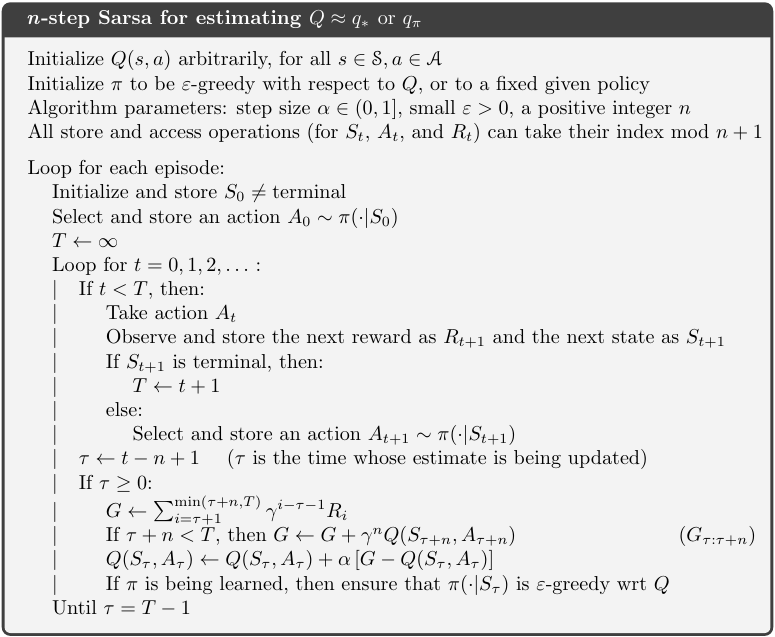
\includegraphics[width=\textwidth]{n-step-sarsa-alg.png}
    \end{frame}

    \section{n-step off Policy Learning}
    \begin{frame}
        \frametitle{n-step Off-Policy Learning}
        \begin{itemize}
            \item Learn from a target policy different from the behavior policy
            \item Importance sampling needed to correct for distribution mismatch
            \item Update rule:
            $$
            Q(s,a) \leftarrow Q(s,a) + \alpha \rho_t \left[G_t^{(n)} - Q(s,a)\right]
            $$
            \item ($\rho_t$): Importance sampling ratio
        \end{itemize}
    \end{frame}

    \begin{frame}{n-step Off-Policy Learning Algorithm}
        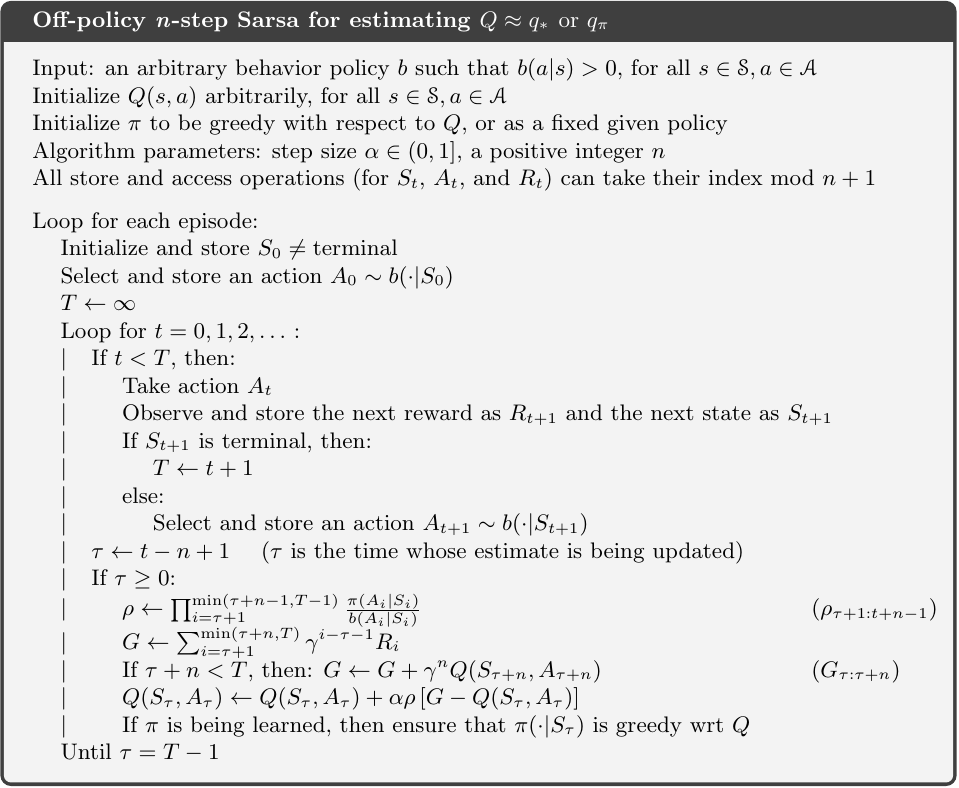
\includegraphics[width=\textwidth]{n-step-offp.png}
    \end{frame}

    \section{Per-decision Methods with Control Variates}
    \begin{frame}
        \frametitle{Per-decision Methods with Control Variates}
        \begin{itemize}
            \item Reduce variance of updates using control variates
            \item Per-decision updates enhance learning stability
            \item Control variates help in adjusting the n-step returns
        \end{itemize}
    \end{frame}


    \section{Off-policy Learning Without Importance Sampling}
    \begin{frame}
        \frametitle{n-step Tree Backup Algorithm}
        \begin{itemize}
            \item Avoids the use of importance sampling ratios
            \item Constructs updates considering multiple future steps
            \item Tree backup algorithm uses:
            $$
            G_t^{(n)} = \sum_{k=0}^{n-1} \gamma^k R_{t+k+1} + \gamma^n \sum_{a} \pi(a|S_{t+n}) Q(S_{t+n}, a)
            $$
        \end{itemize}
    \end{frame}


    \section{A Unifying Algorithm: n-step Q($\sigma$)}
    \begin{frame}
        \frametitle{A Unifying Algorithm: n-step Q($\sigma$)}
        \begin{itemize}
            \item Combines aspects of both n-step SARSA and n-step Tree Backup methods
            \item The parameter \(\sigma\) controls the degree of sampling vs. bootstrapping
            \item Update rule integrates both on-policy and off-policy learning:
            $$
            G_t^{(n)} = (1 - \sigma) \sum_{k=0}^{n-1} \gamma^k R_{t+k+1} + \sigma \sum_{k=0}^{n-1} \gamma^k Q(S_{t+k}, A_{t+k})
            $$
            \item The $(\sigma)$-weighted combination adjusts the algorithm's behavior
            \item Generalizes both the SARSA(λ)-forward view and the Tree Backup algorithm
        \end{itemize}
    \end{frame}
\end{document}